\section{Literature review} \label{sec:litreview}
%Lit. review (actually previous attempts)
%VGG16
%Dahl
%batch norm
%concatenation
%Zhang
%dilation
%classification

\begin{wrapfigure}{R}{0.4\textwidth}
	\vspace{-20pt}
	\begin{center}
		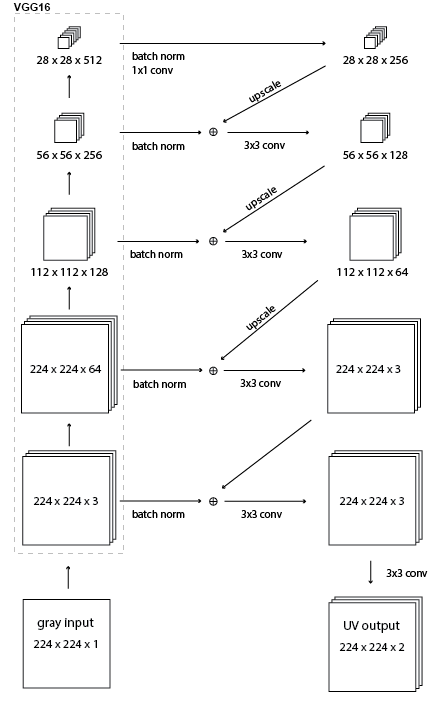
\includegraphics[width=0.35\textwidth]{Dahl_Architecture.png}
	\end{center}
	\caption{Network used by Dahl \cite{Dahl}}
	\label{fig:dahlnetwork}
	\vspace{-20pt}
\end{wrapfigure}

In recent years, Convolutional neural networks (CNN) have become the standard in image
classification \cite{Krizhevsky}. Using a CNN for image colorization is a trend that has emerged only in the past year in the machine learning community. Research from Dahl \cite{Dahl}, Zhang et al. \cite{Zhang}
and Cheng et al. \cite{Cheng} has shown promising results using CNN, however they all use very different
architectures. One of the problems in the image colorization task is the maintainability of spacial information, going back from global features to a special mapping of these features in the detailed image space. 

The use of max-pooling in CNN's makes the network invariant to spatial transformations. However a lot of this information is lost when the final layer of a conventional CNN is reached, which is disadvantageous for a classification and localization task. Different techniques have been proposed to regain a local mapping of the features in the final layers of the network{\color{red} Welke dan?}. 

Another big variation lies in the loss function of the research mentioned previously. Dahl \cite{Dahl} and Zhang et al. \cite{Zhang} both use pre-trained networks for the feature mapping such as VGG16 \cite{Simonyan}, however Cheng et al. \cite{Cheng} completely trains the front-end module of the network from scratch. This offers more flexibility with network architecture, however a lot more computational power is required. 

In this section a short summary of the related work on image colorization using CNN is shown. In addition the paper by \cite{Simonyan} on VGG16 is explained.

\subsection{Dahl}

Dahl \cite{Dahl} is one of the first to use a CNN for image colorization. The network is trained in the YUV colorspace, with the advantage that Y-channel can be used directly as the input of the network. Only the U and V channels will be computed by the network and they are concatenated with the original Y-channel, resulting in a colorized image. This way less information needs to be generated by the network. 
%It is unclear whether the network uses exclusively information from semantic features as opposed to learning color distributions coupled to Y inputs. Zhang et al. \cite{Zhang} have {\color{red}proved} in their network design that this is not the case. 
The pre-trained VGG16 network is used, which already has a large variety of feature extraction. The network is trained on the ImageNet LSVRC 2012 Training Set. 

Maintaining the spatial information is done with the use of partial hypercolumns, also called a residual auto-encoder \cite{hariharan2015hypercolumns}. The image is upscaled by a factor two after each convolutional layer in the output pipeline of the network. These upscaled feature maps are concatenated with the corresponding input layer's feature maps as can be seen in figure \ref{fig:dahlnetwork}. This combination of global and more local features are then convolved using 3x3 convolutional kernels, this process is repeated until all the layers in the front-end are concatenated with the more global features. 

Batch Normalization was applied after each convolutional layer block towards the concatenate layers (see section \ref{sec:batch_norm}). Throughout the network 3x3 convolutional kernels and rectified linear units (ReLu) \cite{nair2010rectified} as non-linearities are used. The loss function consists of applying least squares on the euclidean distance between the target pixel values and the output of the network. Gaussian blur is used over the target output of the image, resulting in better guidance of learning. 

One of the problems encountered is that of color averaging, for images which have a large variety of color probabilities the network chooses the average of these colors. For example, cars can have a large variety of colors. The network colorizes these cars with the mean of all these colors, so in most cases cars will be colored sepia-like. It is proposed to use generative adversarial networks \cite{Radford}, to counter the color averaging problem. Another method to tackle this problem are variational Auto-encoders, altering a direct copy of the output, (variational) auto encoders are described by \cite{Gregor}, \cite{Kingma} and \cite{GoodfellowBOOK}. 


\subsection{Zhang et. al}
Very promising results are obtained by Zang et al. \cite{Zhang}, therefore a lot of the work in this paper is based on their work.
A fully automatic approach is proposed that produces vibrant and realistic colorizations. Again VGG16 is used for feature extraction with some modifications on the input layers. The max-pooling operation is replaced by strides, resulting in less loss of spatial information. 

In the output pipeline of the network, dilated convolutions \cite{yu2015multi} are applied, creating an exponential increasing depth of field with the same number of convolutions compared to conventional convolutional kernels (see figure \ref{fig:dilations}).

\begin{figure}[h]
	\centering
	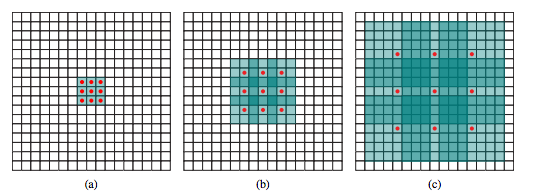
\includegraphics[width=0.63\textwidth]{Dilations}
	\caption{Illustration of dilated convolutions. Figure c shows a receptive field of 15 after only 3 convolutions. Normal convolutions would have a receptive field of 7 after 3 convolutions \cite{yu2015multi}.}
	\label{fig:dilations}
\end{figure}

In addition, the problem is posed as a classification problem, where each output pixel is classified as a certain color. This creates the opportunity of implementing class-rebalancing.
Categorical cross-entropy is applied on the final softmax output layer of the network \cite{de2005tutorial}. The final loss consists out of the categorical cross-entropy loss multiplied with a value function based on the probability of the target color given in equation \ref{eq:lossZhang}, where $h$ and $w$ are the pixel width and height respectively, $Z$ is the target vector, $\widetilde{Z}$ is the output vector, and $v$ is the value function.
Colors which are common in the dataset get a low loss, and colors which are rare in the dataset get a high loss, causing the network to 'steer' towards more saturated colors instead of sepia. 

\begin{equation}
L(\widetilde{Z},Z)=-\frac{1}{HW}\sum_{h,w}v(Z_{h,w})\sum_q^{}{Z_{h,w,q}log({\widetilde{Z}_{h,w,q}})}
\label{eq:lossZhang}
\end{equation}

The colorspace used is CIELab, The L (luminosity) layer is the network input. The CIELab colorspace is discretized into 313 colorbins. Target probabilities per pixel are generated by applying a Gaussian blur on the k-nearest neighbor colorbins. The output of the network consists out of the distribution of probabilities over the colorbins. In order to generate a final choice of colorbin from this output vector, an annealed mean operation is applied on the output probabilities. The temperature T in the annealed mean operation determines whether the mode or the mean of the final distribution is taken as final color. An illustration of the effect of the annealed mean temperature T can be seen in \ref{fig:anmean} This operation is described in more detail in section \ref{sec:method}.

\begin{figure}[h]
\centering
	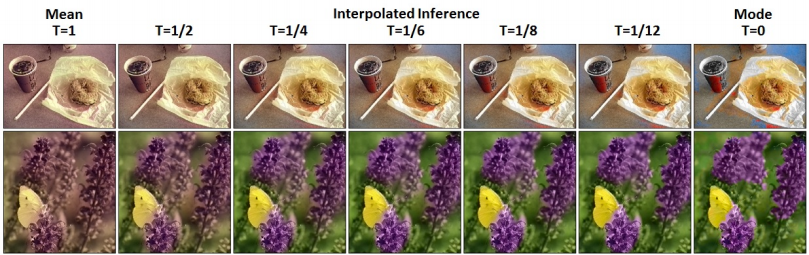
\includegraphics[width=0.8\textwidth]{AnnealedMean}
\centering
\caption{Effect of applying the annealed mean operation on the  color output probabilities of the network \cite{yu2015multi}.}
\label{fig:anmean}
\end{figure}

Various performance measures were applied by Zhang et al, the most interesting one being a 'Turing test' where participants needed to choose between a fake colorization of the image and the true ground colors of the images. The results of Zhang et. al fooled participants in 20.4 \%\ of the cases. 



\subsection{Cheng et al}

\subsection{VGG16}




More literature about convolutional neural networks can be found in \cite{GoodfellowBOOK}. 


%The biggest problem with the machine learning approach to automatic colorization until now, is the case where an object does not have a characteristic color, such as a car or clothing. To solve this problem it is proposed to use generative adversarial networks, to influence the discriminator to be able to generate the right colors where there could be multiple solutions. Generative adversarial networks is described by \cite{Goodfellow} and \cite{Radford}.
%
%The work in this paper is very much an extension to the work of \cite{Dahl}. \cite{Dahl} first converts an RGB image to the YUV colorspace. One of the advantages of the YUV colorspace is that the greyscale values can be used as the Y value. The result of this is that the output of the network, the U and V channels can be concatenated with the input of the network, resulting in a colorized image.

VGG16




Dahl
batch norm
concatenation




Zhang
dilation
classification








\subsection{Batch normalization}\label{sec:batch_norm}
The networks described here all use batch normalization layers, this type of layer is first described in \cite{ioffe2015batch}. During training of deep networks the combination of weights and biases can make the nonlinearities to act in the saturated regime causing problems with vanishing gradient. To overcome this the weights need to be initialized carefully and small learning rates are used resulting in slow convergence. Normalizing the output of intermediate layers with respect to each batch, that is propagated through the network, makes each subpart of the network, separated by batch normalization layers, less sensitive to the weights and biases of the other parts of the network. This results in faster training due to increased learning rates, the weights initialization can be done less carefully and the need for regularization (i.e. dropout) is reduced \cite{ioffe2015batch}.


